\icode{E-MI-MU-L2-261107-002}
（多选）
斜面体 \(A\) 固定在水平地面上，平行于斜面的轻弹簧一端与物块 \(B\) 相连，另一端拴在固定于斜面底端的挡板上。已知斜面倾角为\qty{37}{\degree}，物块 \(B\) 质量 $m_B=$\,\qty{1}{kg}，物块 \(B\) 与斜面间动摩擦因数 $\mu=0.8$，弹簧的原长 $L_0=$\,\qty{20}{cm}，劲度系数 $k=$\,\qty{200}{N/m}，都在弹簧弹性限度内。已知最大静摩擦力等于滑动摩擦力，则物块静止时弹簧的长度不可能的是\paren[]
	
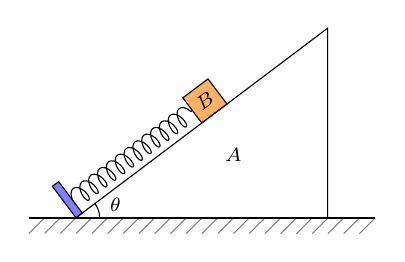
\begin{tikzpicture}[font=\scriptsize]
	\begin{scope}[rotate=37]
		\draw[fill=blue!50] (0,0) rectangle(.1,.5);
		\draw[decoration={aspect=.5,segment length=4,amplitude=1.2mm,coil},decorate] (.1,.2)--(2,.2);
		\draw[fill=orange!60] (2,0) rectangle(2.4,.4)node[midway,rotate=37]{\(B\)};
		\draw (0,0)--(4,0)--++(-127:2.4);
	\end{scope}
	\draw (.3,0) arc(0:37:.3);
	\node at(.5,.16){ \(\theta\)};
	\node at(2,.8){ \(A\)};
	\foreach \x in {-.6,-.4,...,3.8}
		\draw[gray] (\x,-.2)--++(.2,.2);
	\draw[thick] (-.6,0)--(3.8,0);
\end{tikzpicture}
\begin{choices}
	\item \qty{12.8}{cm}
	\item \qty{13.8}{cm}
	\item \qty{20.2}{cm}
	\item \qty{21.2}{cm}
\end{choices}
\begin{answer}
    AD\qquad 提示：
\end{answer}